\documentclass[aspectratio=169]{beamer}
\usepackage{fontspec}
\usefonttheme{professionalfonts}
\usepackage{arydshln}
\usepackage{tikz-cd}
\usepackage[most]{tcolorbox}
\usepackage{subcaption}

\usepackage[backend=bibtex, style=authoryear, doi=false,isbn=false,url=false]{biblatex}
\bibliography{biblio_VKpres}

\usepackage{bm}
\usepackage{color}
\definecolor{theme}{RGB}{0,73,114}

\usepackage{graphicx}
\usepackage{diffcoeff}
\usepackage[most]{tcolorbox}
\usepackage{mathtools}

\usepackage{appendixnumberbeamer}

\setbeamertemplate{caption}{\raggedright\insertcaption\par}

\usepackage[beamer]{hf-tikz}
\usetikzlibrary{calc}


\addtobeamertemplate{footnote}{}{\vspace{2ex}}

\usepackage{xcolor}


% Syntax: \colorboxed[<color model>]{<color specification>}{<math formula>}
\newcommand*{\colorboxed}{}
\def\colorboxed#1#{%
	\colorboxedAux{#1}%
}
\newcommand*{\colorboxedAux}[3]{%
	% #1: optional argument for color model
	% #2: color specification
	% #3: formula
	\begingroup
	\colorlet{cb@saved}{.}%
	\color#1{#2}%
	\boxed{%
		\color{cb@saved}%
		#3%
	}%
	\endgroup
}

% Math macros
\DeclareMathOperator*{\grad}{grad}
\DeclareMathOperator*{\Grad}{Grad}
\DeclareMathOperator*{\Div}{Div}
\renewcommand{\div}{\operatorname{div}}
\DeclareMathOperator*{\Hess}{Hess}
\DeclareMathOperator*{\curl}{curl}
\DeclareMathOperator*{\rot}{rot}
\DeclareMathOperator{\Tr}{Tr}
\DeclareMathOperator{\Dom}{Dom}
\DeclareMathOperator*{\esssup}{ess\,sup}

\newcommand{\bbR}{\mathbb{R}}
\newcommand{\bbF}{\mathbb{F}}
\newcommand{\bbA}{\mathbb{A}}
\newcommand{\bbB}{\mathbb{B}}
\newcommand{\bbS}{\mathbb{S}}

\newcommand*{\norm}[1]{\ensuremath{\left\|#1\right\|}}
\newcommand{\where}{\qquad \text{where} \qquad}


\newcommand{\inpr}[3][]{\ensuremath{( #2, \, #3 )_{#1}}}
\newcommand{\dualpr}[3][]{\ensuremath{\langle #2 \, \vert #3 \rangle_{#1}}}


\newcommand{\pder}[2]{\ensuremath{\partial_{#2} #1}}
\newcommand{\dder}[2]{\ensuremath{\delta_{#2} #1}}
\newcommand{\secref}[1]{\S\ref{#1}}
\newcommand{\energy}[1]{\frac{1}{2} \int_{\Omega} \left\{ #1 \right\} \d\Omega}
\newcommand{\crmat}[1]{\ensuremath{\left[#1\right]_\times}}
\newcommand{\fenics}{\textsc{FEniCS}\xspace}
\newcommand{\firedrake}{\textsc{Firedrake}\xspace}

\DeclareMathOperator*{\argmax}{arg\,max}
\DeclareMathOperator*{\argmin}{arg\,min}

\newtheorem{proposition}{Proposition}
\newtheorem{remark}{Remark}
\newtheorem{hypothesis}{Hypothesis}
\newtheorem{assumption}{Assumption}
\newtheorem{conjecture}{Conjecture}


\def\onedot{$\mathsurround0pt\ldotp$}
\def\cddot{% two dots stacked vertically
	\mathbin{\vcenter{\baselineskip.67ex
			\hbox{\onedot}\hbox{\onedot}}%
}}

\renewcommand\bibfont{\scriptsize}

\setbeamertemplate{navigation symbols}{}

\addtobeamertemplate{navigation symbols}{}{%
	\usebeamerfont{footline}%
	\usebeamercolor[fg]{footline}%
	\hspace{1em}%
	\insertframenumber/\inserttotalframenumber
}

\makeatletter
\g@addto@macro\normalsize{%
	\setlength\abovedisplayskip{5pt}
	\setlength\belowdisplayskip{5pt}
	\setlength\abovedisplayshortskip{5pt}
	\setlength\belowdisplayshortskip{5pt}
}
\makeatother


\makeatletter \renewcommand\d[1]{\ensuremath{%
		\;\mathrm{d}#1\@ifnextchar\d{\!}{}}}
\makeatother

\setbeamertemplate{blocks}[rounded][shadow]

\setbeamercolor{block body alerted}{bg=alerted text.fg!10}
\setbeamercolor{block title alerted}{bg=alerted text.fg!20}
\setbeamercolor{block body}{bg=structure!10}
\setbeamercolor{block title}{bg=structure!20}
\setbeamercolor{block body example}{bg=green!10}
\setbeamercolor{block title example}{bg=green!20}

\graphicspath{{./imagesVK/}}

\newif\iftocsub
\tocsubtrue
\AtBeginSection[] {
	\begin{frame}[noframenumbering]{Outline}
		\tableofcontents[sectionstyle=show/shaded, subsectionstyle=show/show/hide]
	\end{frame}
	\tocsubfalse
}
\AtBeginSubsection[] {
	\iftocsub
	\begin{frame}[noframenumbering]{Outline}
		\tableofcontents[currentsubsection, sectionstyle=show/shaded, subsectionstyle=show/shaded/hide]
	\end{frame}
	\fi
	\tocsubtrue
}

\newcommand{\beginbackup}{
	\newcounter{framenumbervorappendix}
	\setcounter{framenumbervorappendix}{\value{framenumber}}
}
\newcommand{\backupend}{
	\addtocounter{framenumbervorappendix}{-\value{framenumber}}
	\addtocounter{framenumber}{\value{framenumbervorappendix}} 
}


\begin{document}
	
	
	\begin{frame}[plain]
		
		%%%%%%%% Title slide details %%%%%%%%%%%%%%


% Background Image
\newcommand{\myBackground}
{
    \includegraphics[height=1.02\paperheight,page=9]{beamerthemeutresources}
}

% Title
\newcommand{\myTitle}
{
A port-Hamiltonian formulation for the full von-Kármán plate model
}

% Subtitle
\newcommand{\mySubTitle}
{
}

% Author
\newcommand{\myAuthor}   
{
    Andrea Brugnoli and Denis Matignon
}

% Affiliation
\newcommand{\myAffiliate}
{
  
}

% Presentation Date
\newcommand{\myDate}   
{
    18 July 2022
}

% Logo
\newcommand{\myLogo}   
{
    \includegraphics[height=1.5cm]{Logo.png} \hspace{1cm}
    \includegraphics[height=1.5cm]{LogoISAE.png}
}
%%%%%%%%%%%%%%%%%%%%%%%%%%%%%%%%%%%%


%%%%%%%%%% Title slide code %%%%%%%%%%%
\begin{tikzpicture}[remember picture,overlay]

% Background color

\fill[white] (current page.south west) rectangle (current page.north east);
% Background image
\node[above right,inner sep=0pt] at (current page.south west)
    {
        \myBackground
    };
    
% Title & Subtitle
\node
[
    above=0.5cm,
    align=center,
    draw=black!50,
    % rounded corners,
    double,
    double distance=0.1cm,
    double=blue!10,
    fill=theme!10,
    inner xsep=15pt,
    inner ysep=10pt, 
    minimum width=0.8\textwidth,
    text width=0.8\textwidth
] (title) at (current page.center)
{
    \LARGE \myTitle  \\[5pt]
    \small \mySubTitle
};

% Author 
\node[ below=0.5cm] (author) at (title.south){\myAuthor};

% Author 
\node[ below=0.25cm ](affiliate) at (author.south){\small \myAffiliate};

% Date
\node[below=0.25] (date) at (affiliate.south){\large \myDate};

% Logo
\node
[
    below =0.25cm
] at (date.south)
{
    \myLogo
};

\end{tikzpicture}
		
	\end{frame}

	
	\begin{frame}{Outline}
		
		\tableofcontents
		
	\end{frame}

\section{Why port-Hamiltonian systems?}


\begin{frame}{A unified language for multiphysics in engineering}
	The port-Hamiltonian (pH) paradigm provides a language to understand multiphysics:

	\vspace{.3cm}
	
	\begin{columns}
		\begin{column}{.68\textwidth}
			\begin{itemize}
				\item \textbf{Physics} is at the core: pH systems are \textbf{passive} with respect to the \textbf{energy storage function}.
				\item The \textbf{topological} and \textbf{metrical} structure of the equations is clearly separated (mimetic discretization).
				\item PH systems are \textbf{closed under interconnection}. 
			\end{itemize}
		\end{column}
		\begin{column}{.32\textwidth}
			\centering
			\includegraphics[width=.9\columnwidth]{babel_tower.jpeg}
		\end{column}
	\end{columns}

	
\end{frame}


\begin{frame}{Finite dimensional pH systems}
\only<1>{
	\begin{alertblock}{A theory still under developement}
		There is \textbf{not a unique definition} of pH systems, even in finite dimension.
	\end{alertblock}
	
	\begin{definition}[Finite dimensional pH system]
		
		The following time-invariant dynamical system is a pH system
		\begin{equation*}
			\begin{aligned}
				\mathbf{M}\dot{\mathbf{x}} &= \mathbf{J}(\mathbf{x})\mathbf{x} + \mathbf{B}\mathbf{u}, \\
				\mathbf{y} &= \mathbf{B}^\top\mathbf{x}.
			\end{aligned}
		\end{equation*}
		$\mathbf{x}(t) \in \mathcal{X} \subseteq \bbR^n$ is the state, $\mathbf{u}(t), \mathbf{y}(t) \in \bbR^m$ the input and output and
		\begin{itemize}
			\item $\mathbf{J}(\mathbf{x})=-\mathbf{J}(\mathbf{x})^\top \in \bbR^{n \times n}$ the interconnection operator
			\item $\mathbf{B} \in \bbR^{n \times m}$ the control operator.
			\item $H(\mathbf{x}) = \frac{1}{2} \mathbf{x}^\top \mathbf{M} \mathbf{x} : \mathbb{R}^n \rightarrow \mathbb{R}$ with $\mathbf{M} > 0$, the Hamiltonian.
		\end{itemize}
	\end{definition}

}
\only<2>{
\centering
\includegraphics[width=.6\textwidth]{sketch_PH.eps}
}
	
\end{frame}


\begin{frame}{Interconnection of pH systems}

	\only<1>{
		\begin{figure}
			\centering
			\includegraphics[width=.95\textwidth]{sketch_PH_gyrator.eps}
		\end{figure}
	}
	\only<2>{
		\begin{figure}
			\centering
			\includegraphics[width=.95\textwidth]{sketch_PH_transformer.eps}
		\end{figure}
	}
	
\end{frame}

\section{Von-K\'arm\'an theory of thin beams in pH form}

\begin{frame}{Linear vs Von-K\'arm\'an plate theory}

	\begin{columns}
	\begin{column}{.5\textwidth}
			\includegraphics[width=.8\columnwidth]{buckling.jpg}
	\end{column}
	\begin{column}{.5\textwidth}

		Geometrical non-linearities allow describing bifurcations (i.e. buckling).
	\end{column}
	\end{columns}
	
\end{frame}

\begin{frame}{The von-K\'arm\'an assumption}
Second-order approximation of geometrically exact beam/plate theory \textbf{capturing the axial bending coupling.}	

\begin{columns}
	\begin{column}{.5\textwidth}
	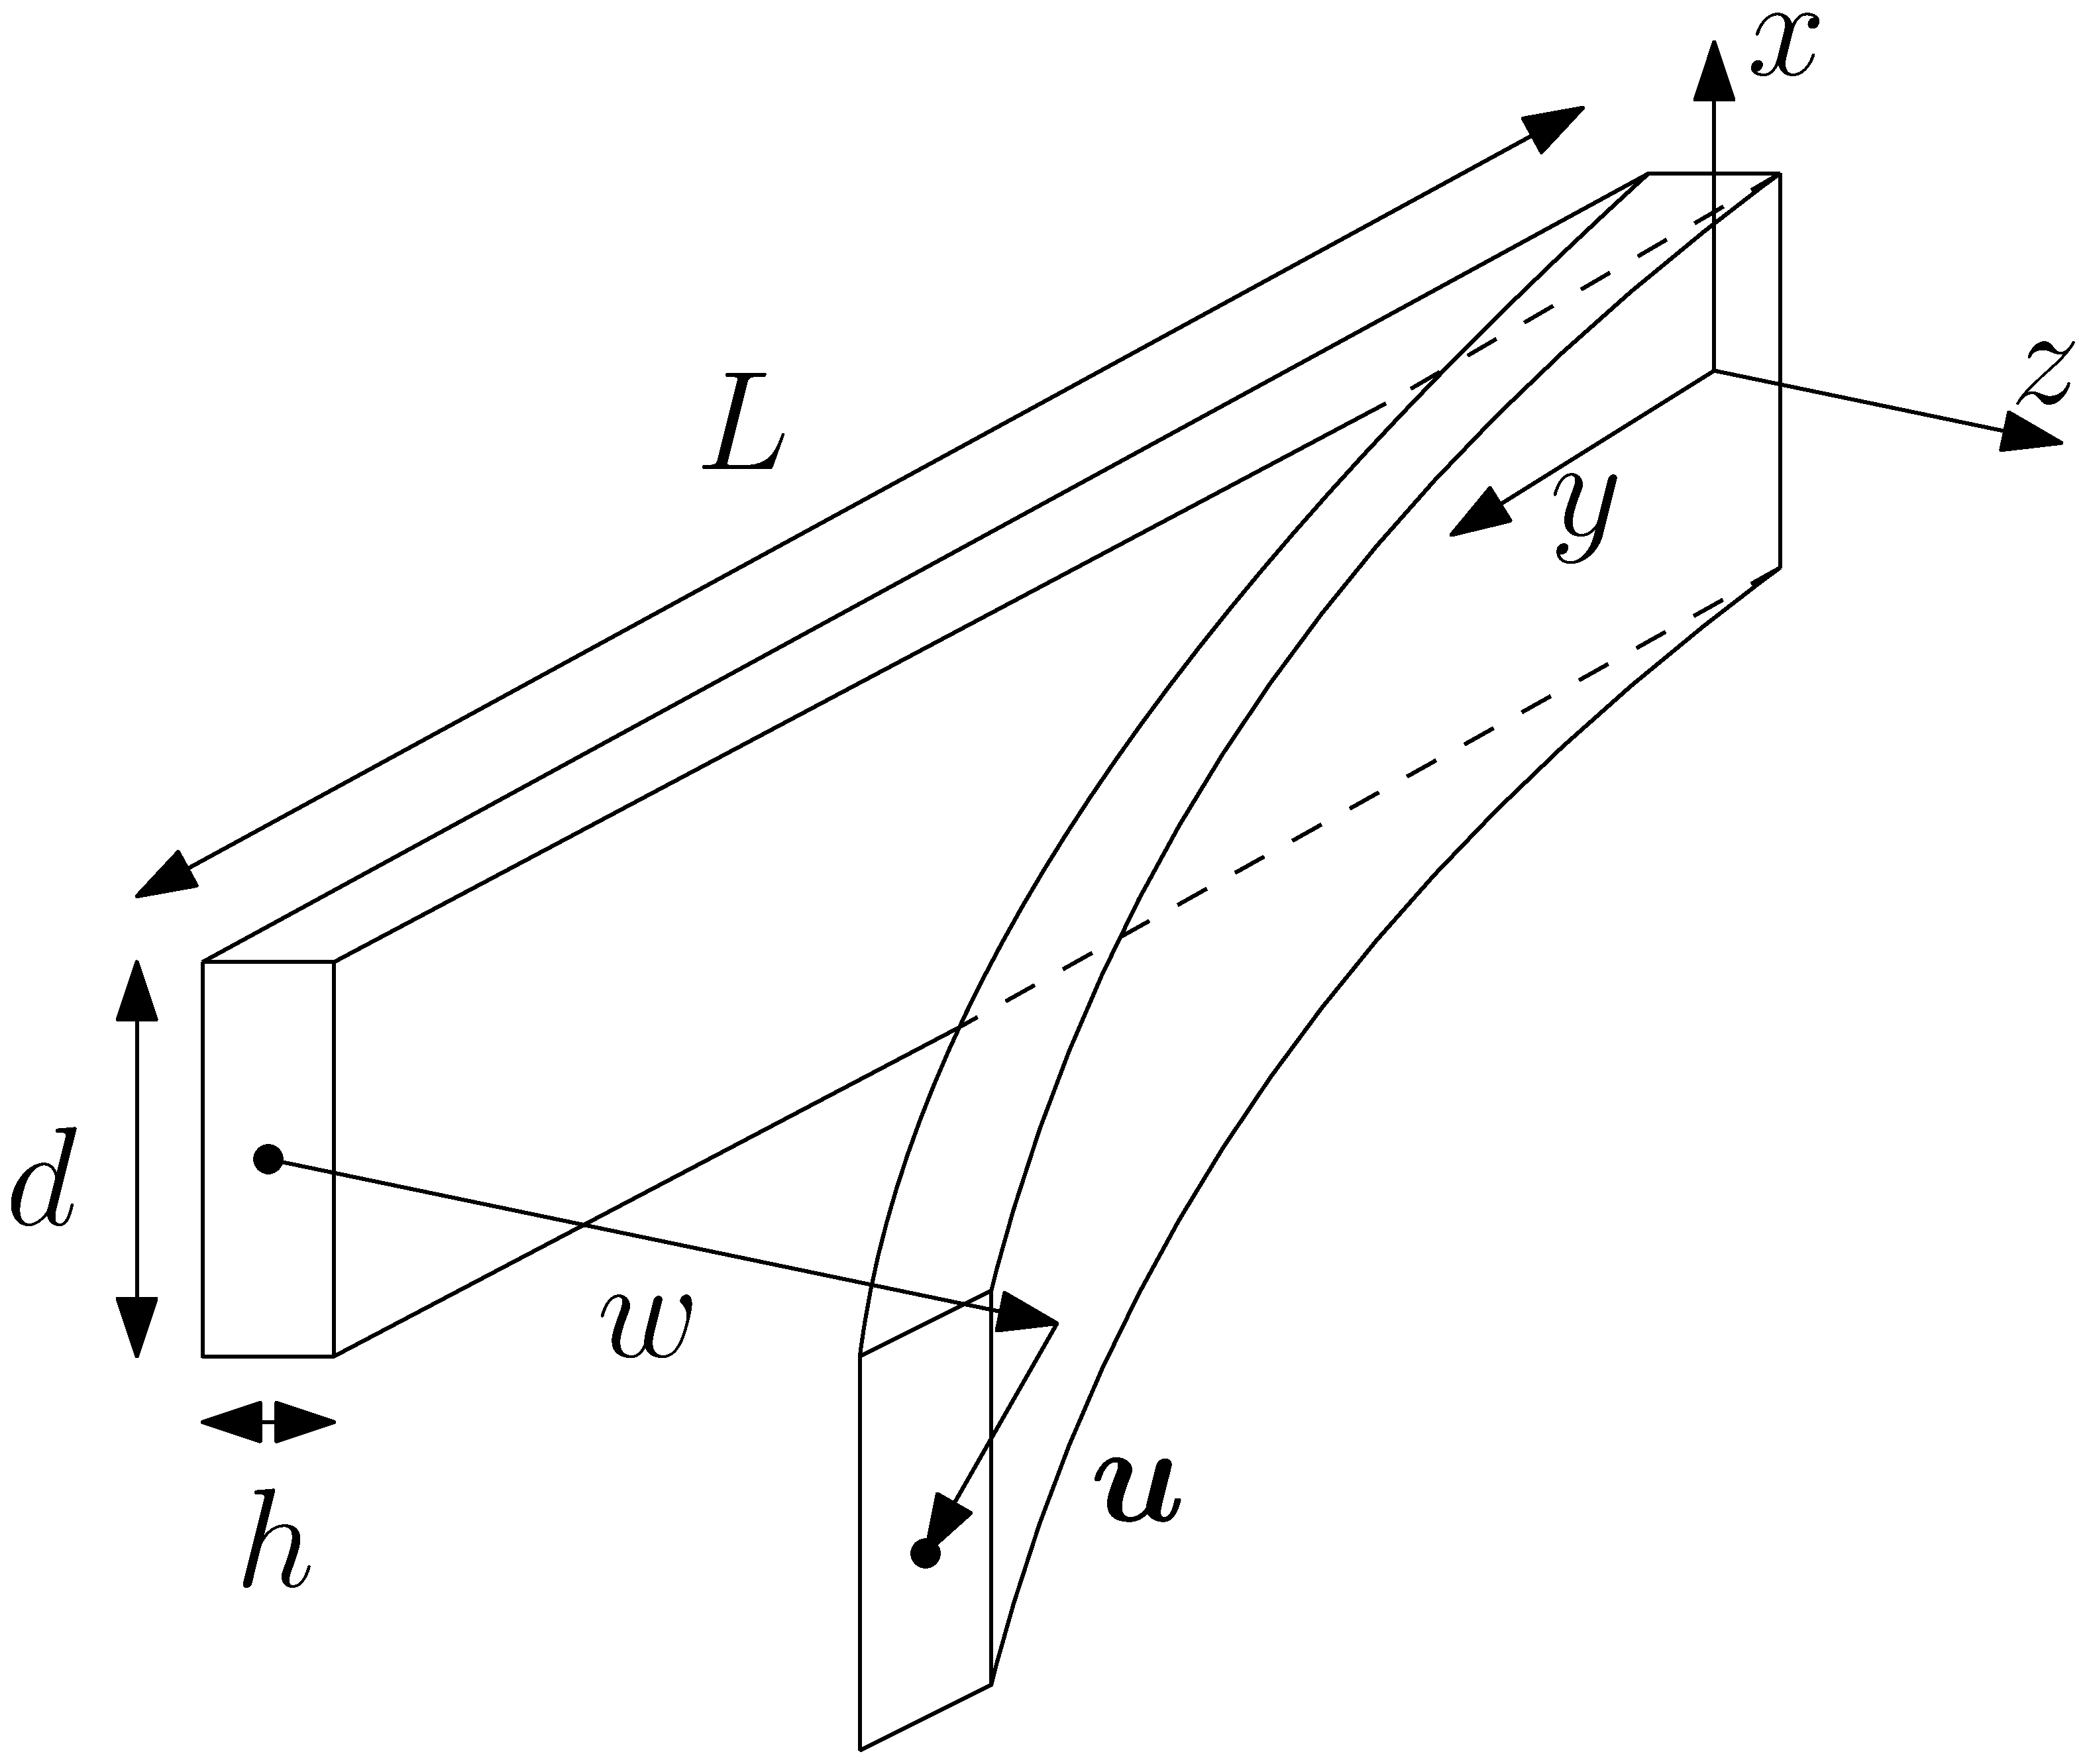
\includegraphics[width=.9\textwidth]{beam_deflected.eps}
	\end{column}
	\begin{column}{.5\textwidth}
	
	\begin{block}{Basic geometric assumptions}
		\begin{itemize}
		\item Out of plane deflection comparable to the thickness: $w/h = \mathcal{O}(1)$.
		\item The squares of the in-plane stretching terms are negligible compared to the square of the rotations.
		\end{itemize}
		
	\end{block}
	
	\end{column}
\end{columns}

\end{frame}


\begin{frame}{Linear isotropic plates ($\Omega \subset \bbR^2$)}
	
	The axial and bending behavior are uncoupled if $w/h \ll 1$:
	
	\begin{tcbraster}[raster columns=2, raster equal height]
		\begin{tcolorbox}[width=0.49\textwidth, nobeforeafter,  colframe=theme,title=Membrane displacement \\
			(2D elastodynamics)]%%
			\begin{equation*}
				\begin{aligned}
				\rho h \partial_{tt} \bm{u} &= \Div \bm{N}, \\
				\bm{N}&=D_m\bm{\Phi}(\bm{\varepsilon}_m), \\
				\bm{\varepsilon}_m &= \mathrm{Sym}(\nabla \bm{u}) = \Grad \bm{u}
				\end{aligned} 
			\end{equation*}
		Total membrane energy
		\begin{equation*}
			\small
			H_m= \frac{1}{2} \int_{\Omega} \rho h ||\partial_t \bm{u}||^2  + D_m \bm{\Phi}(\bm{\varepsilon}_m) \cddot \bm{N} \d\Omega.
		\end{equation*}
		\end{tcolorbox}
		\begin{tcolorbox}[width=0.49\textwidth, nobeforeafter,  colframe=theme,title=Vertical displacement\\ (Kirchhoff plate)]%%
		\begin{equation*}
			\begin{aligned}
				\rho h \partial_{tt} w &= -\div\Div \bm{M}, \\
				\bm{M} &= D_b \bm{\Phi}(\bm{\kappa}), \\
				\bm{\kappa}&= \Hess w = \Grad \grad w. 
			\end{aligned}
		\end{equation*}
		Total bending energy
		\begin{equation*}
			\small
			H_b = \frac{1}{2} \int_{\Omega} \rho h (\partial_t w)^2 + D_b \bm{\Phi}(\bm{\kappa}) \cddot \bm{M} \d\Omega.
		\end{equation*}
		\end{tcolorbox}
	\end{tcbraster}
	
	The linear mapping $\bm\Phi (\bm{A}) = \nu \Tr(\bm{A})\bm{1} + (1 - \nu) \bm{A}$ is positive and preserves symmetry.
	
\end{frame}


\begin{frame}{Von-K\'arm\'an plates}
Decomposition strain field 
\vspace{.3cm}
\begin{equation*}
	\bm{\varepsilon} = \tikzmarkin<1>[below right offset={0.05,-0.4},above left offset={-0.05,0.7}]{lm}\Grad \bm{u}\tikzmarkend{lm} +  \tikzmarkin<1>[below right offset={0,-0.4},above left offset={-0.05,0.7}]{nlm}1/2 \grad w \otimes \grad w\tikzmarkend{nlm} - z \; \tikzmarkin<1>[below right offset={0.05,-0.4},above left offset={-0.05,0.7}]{lb}\Hess w\tikzmarkend{lb} = \bm{\varepsilon}_m -z \bm{\kappa}.
\end{equation*}

\begin{tikzpicture}[remember picture,overlay]
	% adjust the shift from "col" to move the position of the annotation
	\coordinate (lm-a) at ($(lm)+(-1.5,-1.5)$);
	\coordinate (lm-b) at ($(lm)+(0.4,-1.1)$);
	\node[align=left] (lmstring) at (lm-a) {\small{Linear membrane def.}};
	\draw[->, red](lmstring) -| node {} (lm-b);
	
	\coordinate (nlm-a) at ($(nlm)+(-2.2,-2)$);
	\coordinate (nlm-b) at ($(nlm)+(0.8,-1.1)$);
	\node[align=left] (nlmstring) at (nlm-a) {\small{Quadratic membrane def.}};
	\draw[->, red](nlmstring) -| node {} (nlm-b);
	
	\coordinate (lb-a) at ($(lb)+(+2,-2)$);
	\coordinate (lb-b) at ($(lb)+(0.3,-1.1)$);
	\node[align=right] (lbstring) at (lb-a) {\small{Linear bending def.}};
	\draw[->, red](lbstring) -| node {} (lb-b);
\end{tikzpicture}
\vspace{1cm}\\

\begin{block}{Von-K\'arm\'an plate Dynamics}
	\begin{equation*}
		\begin{aligned}
			\rho h \partial_{tt}{u} &= \Div \; \bm{N}, \\
			\rho h \partial_{tt}{w} &= -\div\Div \bm{M} + \div(\bm{N} \grad w),
		\end{aligned} 
	\end{equation*}
Total energy 
$$H= \frac{1}{2} \int_{\Omega} \rho h \{||\partial_t \bm{u}||^2 + ||\partial_t w||^2\} + D_m \bm{\Phi}(\bm{\varepsilon}_m) \cddot \bm{N} + D_b \bm{\Phi}(\kappa)\cddot \bm{M} \d\Omega$$ 
\end{block}

\end{frame}


\begin{frame}{Port-Hamiltonian Von-K\'arm\'an plates}
	
\begin{tcolorbox}[width=0.95\textwidth, nobeforeafter, colframe=theme,title=Energy variables]
The Hamiltonian functional is quadratic in the following variables
\begin{equation*}
	\begin{aligned}
		\bm{\alpha}_u &= \rho h \partial_t \bm{u},\\
		\bm{A}_\varepsilon &= \bm{\varepsilon}_m, \\
	\end{aligned} \quad
	\begin{aligned}
		&\text{Axial momentum},\\
		&\text{Membrane strain}, \\
	\end{aligned} \qquad
	\begin{aligned}
		\alpha_w &= \rho h \partial_t{w}, \\
		\bm{A}_\kappa &= \bm{\kappa},
	\end{aligned}\quad
	\begin{aligned}
		&\text{Bending momentum}, \\
		&\text{Curvature}
	\end{aligned}
\end{equation*}
\end{tcolorbox}
\vspace{.3cm}
\begin{tcolorbox}[width=0.95\textwidth, nobeforeafter, colframe=theme,title=Co-energy variables]
The variational derivative of the Hamiltonian gives the co-energy variables
\begin{equation*}
	\begin{aligned}
		\bm{e}_u &:= \delta_{\bm\alpha_u} H = \dot{\bm{u}},\\
		\bm{E}_\varepsilon &:= \delta_{\bm{A}_\varepsilon} H = D_m \bm{\Phi}(\bm{A}_\varepsilon),
	\end{aligned} \qquad
	\begin{aligned}
		{e}_w &:= \delta_{\alpha_w} H = \dot{w}, \\
		\bm{E}_\kappa &:= \delta_{\bm{A}_\kappa} H = D_b\bm{\Phi}(\bm{A}_\kappa)
	\end{aligned}
\end{equation*}
or more compactly $\bm{e} := \delta_\alpha H = \mathcal{Q} \bm{\alpha}$ with
\begin{equation*}
	\mathcal{Q} = \mathrm{Diag}\left[(\rho h)^{-1}, \; D_m \bm{\Phi}, \; (\rho h)^{-1}, \; D_b \bm{\Phi}\right].
\end{equation*}
\end{tcolorbox}


\end{frame}

\begin{frame}[fragile]\frametitle{The port-Hamiltonian realization}
	
	\begin{equation*}
	\frac{\partial}{\partial t}
	\begin{pmatrix}
		\bm{\alpha}_u \\
		\bm{A}_\varepsilon \\
		\alpha_w \\
		\bm{A}_\kappa
	\end{pmatrix} = 
	\underbrace{\begin{bmatrix}
			\bm{0} & \Div & \bm{0} & \bm{0} \\
			\Grad & \bm{0} & -\mathcal{C}(w)^* & \bm{0} \\
			\bm{0} & \mathcal{C}(w) &  \bm{0} & -\div\Div \\
			\bm{0} & \bm{0} & \Grad\grad & \bm{0} \\ 
	\end{bmatrix}}_{\mathcal{J}}  
	\begin{pmatrix}
		\delta_{\bm\alpha_u} H \\
		\delta_{\bm{A}_\varepsilon} H \\
		\delta_{\alpha_w} H \\
		\delta_{\bm{A}_\kappa} H
	\end{pmatrix}.
\end{equation*}
The operator $\mathcal{J}$ is formally skew-adjoint. \\
The coupling term reads
\begin{equation*}
	\begin{aligned}
		\mathcal{C}(w)(\cdot): L^2(\Omega; \bbR^{2\times 2}_{\text{sym}}) \rightarrow L^2(\Omega), \\
								\bm{X}  \rightarrow \div( \bm{X} \grad w), \\
	\end{aligned} 
\end{equation*}
and its formal adjoint
\begin{equation*}
	\begin{aligned}
		\mathcal{C}(w)^*(\cdot): L^2(\Omega) \rightarrow L^2(\Omega; \bbR^{2\times 2}_{\text{sym}}), \\
		y  \rightarrow  -\mathrm{Sym}\left[\grad (y) \otimes \grad(w)\right].
	\end{aligned}
\end{equation*}


\end{frame}

\begin{frame}{Pure coenergy formulation}
	
	\begin{tcolorbox}[nobeforeafter, colframe=theme,title=Incorporation of the constitutive equations]
		Once the $\mathcal{Q}$ operator (matrix) is inverted, the dynamics is expressed :
		\begin{equation*}
			\begin{pmatrix}
				\rho h\partial_t \bm{e}_u \\
				(D_m \bm{\Phi})^{-1} \partial_t \bm{E}_\varepsilon \\
				\rho h\partial_t e_w \\
				(D_b \bm{\Phi})^{-1} \partial_t \bm{E}_\kappa
			\end{pmatrix} = 
			\begin{bmatrix}
				\bm{0} & \Div & \bm{0} & \bm{0} \\
				\Grad & \bm{0} & -\mathcal{C}(w)^* & \bm{0} \\
				0 & \mathcal{C}(w) & 0 & -\div\Div \\
				\bm{0} & \bm{0} & \Grad\grad & \bm{0} \\ 
			\end{bmatrix}
			\begin{pmatrix}
				\bm{e}_u \\
				\bm{E}_\varepsilon \\
				e_w \\
				\bm{E}_\kappa
			\end{pmatrix},
		\end{equation*}
		where the vertical position is given by 
		\begin{equation*}
		w(t) = w_0 + \int_0^t e_w(\tau) \d\tau.
		\end{equation*}
	\end{tcolorbox}

	
\end{frame}


\begin{frame}{Energy rate and boundary conditions}
	
	\begin{proposition}{The energy rate reads}
	\begin{equation*}
		\dot{H} = \dualpr[\partial\Omega]{\gamma_0\bm{e}_u}{\gamma_\perp \bm{E}_\varepsilon} + \dualpr[\partial\Omega]{\gamma_0\bm{e}_w}{\gamma_{\perp\perp, 1} \bm{E}_\kappa + \gamma_0(\bm{E}_\varepsilon \bm{n} \cdot \grad w)} + \dualpr[\partial\Omega]{\gamma_1\bm{e}_w}{\gamma_{\perp\perp} \bm{E}_\kappa},
	\end{equation*}
\begin{itemize}
	\item $\gamma_0\bm{e}_u= \bm{e}_u\vert_{\partial\Omega}$ is the Dirichlet trace;
	\item $\gamma_\perp \bm{E}_\varepsilon = \bm{E}_\varepsilon \bm{n}\vert_{\partial\Omega}$ is the normal trace;
	\item $\gamma_{\perp\perp, 1} \bm{E}_\kappa = - \bm{n} \cdot \Div \bm{E}_\kappa - \partial_{\bm{s}}(\bm{n}^\top \bm{E}_\kappa \bm{s})\vert_{\partial\Omega}$ is the effective shear force;
	\item $\gamma_1 \bm{e}_w = \partial_{\bm{n}} \bm{e}_w\vert_{\partial\Omega}$ is the normal derivative trace;
	\item $\gamma_{\perp\perp} \bm{E}_\kappa = \bm{n}^\top \bm{E}_\kappa \bm{n}$ is the normal to normal trace.
\end{itemize}
	\end{proposition}

\begin{table}[h]
	Boundary conditions classification
	\centering
	\begin{tabular}{c|c|c|c}
		\hline 
		BCs & Traction & \multicolumn{2}{c}{Bending} \\ 
		\hline 
		Kinematical/Dirichlet & $\gamma_0 \bm{e}_u$ & $\gamma_0\bm{e}_w$  & $\gamma_1 \bm{e}_w $  \\
		Dynamical/Neumann & $\gamma_\perp \bm{E}_\varepsilon$ & $\gamma_{\perp\perp, 1} \bm{E}_\kappa + \gamma_0(\bm{E}_\varepsilon \bm{n} \cdot \grad w)$ & $\gamma_{\perp\perp} \bm{E}_\kappa$ \\ 
		\hline 
	\end{tabular} 
\end{table}

\end{frame}


\section{Numerical discretization}

\begin{frame}[fragile]\frametitle{Mixed finite elements for elasticity}
	Crucial concept to derive stable convergent approximations: \textbf{Hilbert complexes}.
	
	\begin{figure}
		\centering
		\begin{tikzcd}
			H^1(\Omega) \arrow[r, "\grad"] \arrow[d, "\Pi_{s, h}^{-, 0}"]
			& H^{\curl}(\Omega) \arrow[r, "\curl"] \arrow[d, "\Pi_{s, h}^{-, 1}"] & H^{\div}(\Omega) \arrow[r, "\div"] \arrow[d, "\Pi_{s, h}^{-, 2}"]
			& L^2(\Omega) \arrow[d, "\Pi_{s, h}^{-, 1}"] \\
			\mathrm{CG}_s(\Omega_h) \arrow[r, "\grad"] 
			& \mathrm{NED}_s^1(\Omega_h) \arrow[r, "\curl"] & \mathrm{RT}_s(\Omega_h) \arrow[r, "\div"]
			& \mathrm{DG}_{s-1}(\Omega_h) 
		\end{tikzcd}  
			\includegraphics[width=.75\textwidth]{Whitney.png}
		\caption*{The Whitney forms $s=0$ form a subcomplex of the de Rham complex}
	\end{figure}
	This framework is well developed for linear problems \footfullcite{arnold2006acta} and open source finite elements libraries implement them. 	Definitely less for non linear elasticity problems. \vspace{.2cm}
	
\end{frame}

\begin{frame}[fragile]\frametitle{Weak formulation for 2D Elastodynamics}
	
\begin{tcolorbox}[nobeforeafter, colframe=theme,title=$\Grad$ primal formulation]%%
	Suppose the traction (Neumann) boundary condition $\gamma_\perp\bm{E}_\varepsilon = \bm{g}_N$.\\
	Find $\bm{e}_u \in H^1(\Omega; \bbR^2), \; \bm{E}_{\varepsilon} \in H(\rot\rot, \Omega; \bbR^{2\times 2}_{\text{sym}})$ \\
	such that $\forall \bm{\psi}_u \in H^1(\Omega; \bbR^2), \; \forall \bm{\Psi}_\varepsilon \in H(\rot\rot, \Omega; \bbR^{2\times 2}_{\text{sym}})$ the following holds
	\begin{equation*}
		\begin{aligned}
			\inpr[\Omega]{\bm{\psi}_u}{\rho h \partial_t \bm{e}_u} &= -\inpr[\Omega]{\Grad \bm{\psi}_u}{\bm{e}_u} + \dualpr[\partial\Omega]{\gamma_0\bm{\psi}_u}{\bm{g}_N}, \\
			\inpr[\Omega]{\bm{\Psi}_\varepsilon}{(D_m \bm{\Phi})^{-1} \partial_t \bm{E}_{\varepsilon}} &= \inpr[\Omega]{\bm{\Psi}_\varepsilon}{\Grad \bm{e}_u}.
		\end{aligned}
	\end{equation*}
 
\vspace{.5cm}

This formulation is related to the strain elasticity complex in 2D 
\begin{figure}[h]
	\centering
	\begin{tikzcd}
		H^1(\Omega; \bbR^2) \arrow[r, "\Grad"]
		& H(\rot\rot, \Omega; \bbR^{2\times 2}_{\text{sym}}) \arrow[r, "\rot\rot"]  & L^2(\Omega).
	\end{tikzcd}  
\end{figure}
\end{tcolorbox} 


\end{frame}

\begin{frame}[fragile]\frametitle{Weak formulation for 2D Elastodynamics}
		
	\begin{tcolorbox}[nobeforeafter, colframe=theme,title=$\Div$ dual formulation]%%
		Suppose the kinematic (Dirichlet) boundary condition $\gamma_0 \bm{e}_u = \bm{g}_D$. \\
		Find $\bm{e}_u \in L^2(\Omega; \bbR^2), \; \bm{E}_{\varepsilon} \in H(\Div, \Omega; \bbR^{2\times 2}_{\text{sym}})$ \\
		such that $\forall \bm{\psi}_u \in L^2(\Omega; \bbR^2), \; \forall \bm{\Psi}_\varepsilon \in H(\Div, \Omega; \bbR^{2\times 2}_{\text{sym}})$ the following holds
		\begin{equation*}
			\begin{aligned}
				\inpr[\Omega]{\bm{\psi}_u}{\rho h \partial_t \bm{e}_u} &= \inpr[\Omega]{\bm{\psi}_u}{\Div\bm{E}_{\varepsilon}}, \\
				\inpr[\Omega]{\bm{\Psi}_\varepsilon}{(D_m \bm{\Phi})^{-1} \partial_t \bm{E}_{\varepsilon}} &= -\inpr[\Omega]{\Div \bm{\Psi}_\varepsilon}{ \bm{e}_u} + \dualpr[\partial\Omega]{\gamma_\perp \bm{E}_\varepsilon}{\bm{g}_D}.
			\end{aligned} 
		\end{equation*}
	\vspace{.5cm}
	
	This formulation is related to the Elasticity complex in 2D 
	\begin{figure}[h]
		\centering
		\begin{tikzcd}
			H^2(\Omega) \arrow[r, "\curl\curl"]
			& H(\Div, \Omega; \bbS) \arrow[r, "\Div"]  & L^2(\Omega; \bbR^2).
		\end{tikzcd}  
	\end{figure}
	\end{tcolorbox} 

\end{frame}


\begin{frame}{Finite element complexes}
Semi discretization in space is obtained using finite elements forming a \textbf{subcomplex of original Hilbert complex}. But the theory is still under development\footfullcite{chen2022finite} and no open source software. \\
\vspace{1cm}
So heuristic choice of the finite elements.
\end{frame}



\begin{frame}{Finite element choice and final system}
	For the proposed weak formulation, the FE spaces become
	\begin{equation*}
			\bm{e}_u^h \in \mathrm{CG}_{2s-1}, \qquad
			\bm{E}_{\varepsilon}^h \in \mathrm{DG}_{2s-2}, \qquad 
			e_w^h \in \mathrm{CG}_{s}, \qquad \bm{E}_\kappa^h \in \mathrm{HHJ}_{s-1}, \quad s\ge 1.
	\end{equation*}

\begin{equation*}
	\begin{aligned}
		\inpr[\Omega]{\bm{\psi}_u^h}{\rho h \partial_t \bm{e}_u^h} &= -\inpr[\Omega]{\Grad \bm{\psi}_u^h}{\bm{e}_u^h}, \\
		\inpr[\Omega]{\bm{\Psi}_\varepsilon^h}{(D_m \bm{\Phi})^{-1} \partial_t \bm{E}_{\varepsilon}^h} &= \inpr[\Omega]{\bm{\Psi}_\varepsilon^h}{\Grad \bm{e}_u^h} + \inpr[\Omega]{\bm{\Psi}_\varepsilon^h}{\mathrm{Sym}\{\grad e_w^h \otimes \grad w^h\}}, \\
		\inpr[\Omega]{\psi_w^h}{\rho b \partial_t {e}_w^h} &= +d_h(\psi_w^h, \ \bm{E}_{\kappa}^h) - \inpr[\Omega]{\mathrm{Sym}\{\grad \psi_w^h \otimes \grad w^h\}}{\bm{E}_\varepsilon^h}, \\ 
		\inpr[\Omega]{\bm{\Psi}_\kappa^h}{(D_b \bm{\Phi})^{-1}\partial_t {\bm{E}}_\kappa^h} &= -d_h(e_w^h, \ \bm{\Psi}_{\kappa}^h). \\ 
	\end{aligned}
\end{equation*}

\begin{block}{Finite dimensional system (Galerkin projection)}
		\begin{equation*}
		\begin{aligned}
			\mathbf{M} \dot{\mathbf{e}} &= \mathbf{J}(\mathbf{w})\mathbf{e} + \mathbf{B}\mathbf{u}, \\
			\dot{\mathbf{w}} &= \begin{bmatrix}
				\mathbf{0} & \mathbf{0} & \mathbf{I} & \mathbf{0} \\
			\end{bmatrix} \mathbf{e}, \\
			\mathbf{y} &= \mathbf{B}^\top \mathbf{e}.
		\end{aligned}
	\end{equation*}
\end{block}

\end{frame}


\section{Numerical convergence study}

\begin{frame}{Manufactured solution}
	Consider $\Omega= [0,1] \times [0, 1]$. The following manufactured solution is considered
	\begin{equation*}
		\begin{aligned}
			\bm{u}^{\text{ex}} &= \begin{pmatrix}
				x^4 (1-x^4)\sin^2(\pi y) \\
				\sin^2(\pi x) y^4 (1-y^4)
			\end{pmatrix} \sin(2\pi t), \qquad
			w^{\text{ex}} &= \sin(\pi x)\sin(\pi y)\sin(2 \pi t), 
		\end{aligned}
	\end{equation*}
	together with the boundary conditions
	\begin{equation*}
		\bm{u}|_{\partial\Omega} = 0, \quad w|_{\partial\Omega}=0, \quad \bm{n}^\top\bm{M}\bm{n}|_{\partial\Omega}=0.
	\end{equation*}
A Crank-Nicholson scheme is used for time integration.
\begin{block}{Convergence measure}
	The discrete time-space norm $L^\infty_{\Delta t} (\mathcal{X}) (\mathcal{X} = H^1 \text{or } L^2)$ is used to measure convergence
	\[
	||\cdot ||_{L^\infty (\mathcal{X})} \approx || \cdot ||_{L^\infty_{\Delta t} (\mathcal{X})} = \max_{t \in t_i} ||\cdot||_{\mathcal{X}},
	\]
	where $t_i$ are the discrete simulation instants.
\end{block}

\end{frame}

\begin{frame}{Results}
	\only<1>{
		\begin{figure}[b]
				\centering
				\includegraphics[width=.7\textwidth]{u_dot.eps}
				\caption{$L^\infty_{\Delta t} (H^1)$ error for $e_u$.}
		\end{figure}
	}
	\only<2>{
		\begin{figure}[b]
				\centering
				\includegraphics[width=.7\textwidth]{N_tens.eps}
				\caption{$L^\infty_{\Delta t} (L^2)$ error for $e_\varepsilon$.}
		\end{figure}
	}
	\only<3>{
		\begin{figure}[b]
				\centering
				\includegraphics[width=.7\textwidth]{w_dot.eps}
				\caption{$L^\infty_{\Delta t} (H^1)$ error for $e_w$.}
		\end{figure}
	}
	\only<4>{
		\begin{figure}[b]
				\centering
				\includegraphics[width=.7\textwidth]{M_tens.eps}
				\caption{$L^\infty_{\Delta t} (H^1)$ error for $e_\kappa$.}
		\end{figure}
	}
\end{frame}

\begin{frame}{Conclusion and Outlook}
\begin{itemize}
	\item First step into pH non linear mechanics. The \textbf{geometrical non linearities} belong to the \textbf{interconnection operator}.
	\item Can be used to study more complex phenomena. The discretization method guarantees \textbf{exact discrete energy conservation} when \textbf{symplectic time integration} is used.
	\item \textbf{System theory perspective}: incorporates \textbf{interactions} with the environment by means of the \textbf{boundary conditions}.
\end{itemize}
\end{frame}

\appendix

\begin{frame}[allowframebreaks]{References}\label{lastslide}
	\printbibliography
\end{frame}


\begin{frame}[fragile]\frametitle{Mixed finite element construction: Kirchhoff plate}
	
	
	Find $(e_w, \bm{E}_\kappa) \in \mathrm{CG}_s \times \mathrm{HHJ}_{s-1}$ such that
	\begin{equation*}
		\begin{aligned}
			\inpr[\Omega]{\psi_w}{\rho b \partial_t {e}_w} &= +d_h(\psi_w, \ \bm{E}_{\kappa}), \\ 
			\inpr[\Omega]{\bm{\Psi}_\kappa}{(D_b \bm{\Phi})^{-1}\partial_t {\bm{E}}_\kappa} &= -d_h(e_w, \ \bm{\Psi}_{\kappa}), \\ 
		\end{aligned} \qquad
		\begin{aligned}
			\forall \; \psi_w &\in \mathrm{CG}_s, \\
			\forall \; \bm{\Psi}_{\kappa} &\in \mathrm{HHJ}_{s-1}. \\
		\end{aligned}
	\end{equation*}
This method is non-conforming and includes inter-cells terms
	\begin{equation*}
		d_h(v_w, \ \bm{E}_{\kappa}) := - \sum_{T \in \mathcal{T}_h} \inpr[\Omega]{\Hess v_w}{\bm{E}_\kappa} + \sum_{E \in \mathcal{E}_h} \inpr[\Omega]{[\![\partial_n v_w]\!]}{\bm{n}^\top\bm{E}_\kappa \bm{n}}. 
	\end{equation*}
	
	The $\div\Div$ distributional complex in 2D and the HHJ finite element complex:
	\begin{figure}[h] 
		\centering
		\begin{tikzcd}
			H^1(\Omega; \bbR^2) \arrow[r, "\mathrm{Sym}\curl"] \arrow[d, "\bm{I}_h"]
			& H^{-1}(\div\Div, \Omega; \bbR^{2\times 2}_{\text{sym}}) \arrow[r, "\div\Div"] \arrow[d, "\bm{\Pi}_h"]  & L^2(\Omega) \arrow[d, "Q_h"] \\ 
			\mathrm{CG}_s \arrow[r, "\mathrm{Sym}\curl"]
			& \mathrm{HHJ}_{s-1} \arrow[r, "\div\Div_h"]  & \mathrm{CG}_s, \\ 
		\end{tikzcd}  
	\end{figure}
\end{frame}


\end{document}

